\documentclass[10pt,twocolumn]{article}

\usepackage[margin=0.72in]{geometry}
\usepackage{amsmath,amssymb}
\usepackage{booktabs}
\usepackage{graphicx}
\usepackage{microtype}
\usepackage{xcolor}
\usepackage{hyperref}
\usepackage{enumitem}

\hypersetup{colorlinks=true,linkcolor=blue,citecolor=blue,urlcolor=blue}
\graphicspath{{figures/}}

\title{Selective Semantic Correspondence under Real RGB-D Domain Shift: \\
Separating Candidate Availability from Pose Recovery}
\author{Anonymous Authors}
\date{}

\newcommand{\ours}{\textsc{SelectiveMatch}}

\begin{document}
\maketitle

\begin{abstract}
Pose-free correspondence across independently captured RGB-D scans is often
evaluated as if semantic matching and rigid registration were the same problem.
We separate these objectives. Our method concatenates shallow, middle, and deep
frozen DINOv2 patch tokens, retains top-$K$ reference candidates, and uses 3-D
spatial-consensus RANSAC to identify globally coherent correspondences without
using the query-to-reference alignment during matching. On the original
14-pair matched subset, the ViT-G point estimate of retained-set semantic
accuracy rises from 85.1\% to 86.9\% over ViT-L/14, but the pair-bootstrap
interval includes zero; the expanded 16-source ViT-G audit reaches 85.0\%
while explicit candidate-set and wrong-pose failures remain.
On one held-out target, ViT-G reaches 68.0\%
inlier coverage, 93.5\% semantic inlier accuracy, and $1.54^\circ$ rotation
error. A source-only residual gate fit to a requested 90\% retained semantic
accuracy on source queries retains 22.1\% of target queries at 96.6\% retained
semantic accuracy.
Its target semantic mIoU is 89.5\% conditional on retained queries, versus
19.7\% over the fixed query population when abstentions count as false negatives.
Cross-fitted
pooling over all 16 held-out source folds retains only 9.1\% of queries at
76.6\% retained semantic accuracy, so the source-fit operating point is not a
universal guarantee.
We argue that correspondence quality, pose recovery, and abstention coverage
should be reported separately, and make the failure taxonomy part of the
result.
\end{abstract}

\section{Introduction}

Matching observations from independently captured RGB-D scans is useful for
semantic map transfer, object retrieval, and 3-D scene understanding. The
problem is deceptively easy to overstate: a correspondence can have the right
semantic category while supporting a wrong global rigid transform, and a
correct transform can have too few semantically useful matches. We therefore
ask a narrower and testable question:
\emph{can a frozen visual descriptor plus spatial verification expose a useful
subset of cross-scan semantic correspondences with high retained semantic accuracy?}

We study this question on annotated 3RScan reference/rescan pairs
\cite{3rscan}. The method uses no known alignment while selecting candidates.
It concatenates tokens from three transformer depths of a frozen DINOv2
backbone \cite{dinov2}, keeps top-$K$ reference candidates per query, and
selects a spatially coherent hypothesis with 3-point RANSAC
\cite{ransac}. The resulting
residual and inlier status provide an abstention mechanism. We evaluate semantic
and instance label transfer separately from rigid pose error, and compare with
classical FPFH \cite{fpfh} and learned FCGF \cite{fcgf} geometry-only
baselines.

Figure~\ref{fig:method} summarizes the matching path and makes the separation
between matching-time inputs and evaluation-only alignment explicit.

Our central finding is deliberately asymmetric. ViT-G gives a higher
point estimate of final retained-set semantic accuracy on the matched subset,
but the interval includes zero and the experiment does not isolate a
pre-consensus candidate-layer scale effect. The complete source
audit contains pairs where even the most spatially consistent candidates are
wrong. The strongest
claim supported by the evidence is therefore \emph{selective semantic
correspondence}, not universal pose-free registration.

\paragraph{Positioning.}
Our setting sits between frozen visual representation learning and classical
3-D registration. DINOv2 provides the appearance descriptor, while FPFH and
FCGF represent geometry-only local descriptors; the latter is a learned
baseline trained for geometric matching rather than semantic identity
\cite{fpfh,fcgf}. We focus on the evaluation gap that remains after candidate
retrieval: semantic correctness, rigid-pose validity, and abstention coverage
are measured as separate outcomes rather than collapsed into one registration
score.

Our contributions are:
\begin{enumerate}[leftmargin=1.5em,itemsep=1pt]
  \item a pose-free top-$K$ candidate and spatial-consensus protocol that
  separates semantic correspondence from global pose recovery;
  \item a controlled ViT-L to ViT-G scale-up on an original 14-pair subset,
  followed by a 17-pair ViT-G audit, and classical FPFH plus learned FCGF
  geometry-only controls;
  \item a source-only risk--coverage and empirical source-fit gate audit with explicit
  candidate-availability, wrong-consensus, and wrong-pose failure cases; and
  \item a downstream cross-scan semantic/instance label-transfer evaluation
  with class-balanced mIoU.
\end{enumerate}

\section{Related Work}

\paragraph{Learned 3-D correspondence and registration.}
Geometry-first methods such as 3DMatch~\cite{3dmatch} and FCGF~\cite{fcgf}
learn local descriptors for partial-scan matching, while PointDSC~\cite{pointdsc}
and GeoTransformer~\cite{geotransformer} use spatial structure to improve
outlier rejection or registration. REGTR~\cite{regtr} further predicts
correspondences with a transformer rather than relying on a hand-designed
matching stage. These methods primarily optimize geometric inlier quality or
registration recall. We instead use frozen RGB tokens to test semantic
semantic candidate quality under scan shift, and treat pose recovery as a separate
outcome. The FPFH and FCGF rows in our experiments therefore serve as
geometry-only controls, not as claims of state-of-the-art geometric
registration.

Recent 3-D foundation models make the boundary worth stating explicitly:
DUSt3R~\cite{dust3r} and MASt3R~\cite{mast3r} infer pointmaps or image-level
matches, while VGGT~\cite{vggt} predicts scene geometry and 3-D tracks from
RGB views. Their inputs, outputs, and standard protocols differ from our
native-coordinate RGB-D, post-hoc semantic-label-transfer setting, so we do
not present them as directly comparable baselines. Semantic-aware registration
methods such as SemReg~\cite{semreg} and ML-SemReg~\cite{mlsemreg} are also
adjacent: they train semantic/geometric registration models, whereas our
descriptor is frozen and labels are used only for evaluation.

\paragraph{Visual features and semantic transfer.}
Large self-supervised visual features such as DINOv2~\cite{dinov2} provide
strong appearance representations without task-specific correspondence
training. Our use of DINOv2 is intentionally frozen: the contribution is the
candidate--consensus evaluation protocol and its selective operating point,
rather than a new descriptor-training objective. In particular, semantic
agreement can remain high when a globally incorrect pose is selected, so a
registration recall number alone is insufficient for the cross-scan label
transfer setting studied here.

\begin{figure*}[t]
\centering
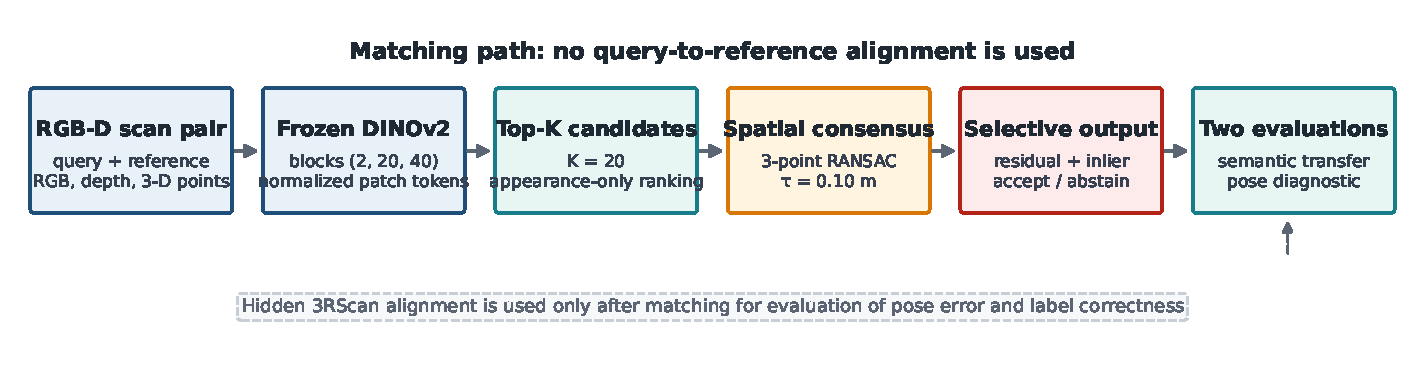
\includegraphics[width=0.98\textwidth]{method_pipeline.pdf}
\caption{The pose-free matching path. Frozen multi-scale tokens produce a
top-$K$ candidate set, spatial consensus selects a coherent hypothesis, and
residuals expose a selective accept/abstain decision. The hidden 3RScan
alignment is used only after matching for evaluation; annotation availability
is not used to construct candidate sets.}
\label{fig:method}
\end{figure*}

\section{Method}

\subsection{Multi-scale candidate descriptors}
For each RGB-D frame, we resize RGB with bilinear interpolation and depth with
nearest-neighbor interpolation to $224\times224$ pixels, scale the complete
intrinsic rows accordingly, and convert depth to meters. We sample the first
20 frames in manifest order from each side (the same 20-reference/20-rescan
protocol for every headline pair). At each 14-pixel patch center with finite,
positive depth, we back-project into the native scan coordinate frame and
retain the point even when its annotation is missing. No 3-D point deduplication
is applied across frames. RGB is ImageNet-normalized before frozen DINOv2
inference. For ViT-G/14, each selected block token is $\ell_2$-normalized,
the $(2,20,40)$ tokens are concatenated, and the concatenation is normalized
once more. Let $q_i$ denote a query patch descriptor and $r_j$ a reference
descriptor. We retain the top-$K$ candidates
\[
  \mathcal{C}_i = \operatorname{TopK}_j\; q_i^\top r_j,
\]
with $K=20$. The alignment between the two scans is not used in this stage.

\subsection{Spatial consensus}
Let $x_i\in\mathbb{R}^3$ be a query point in native rescan coordinates and
$y_j\in\mathbb{R}^3$ a reference point in native reference coordinates.
The transform $T_{qr}=(R,t)$ maps query to reference coordinates. For a
candidate set $\mathcal{C}_i$ of reference indices, we define
\[
  \hat j_i(T)=\arg\min_{j\in\mathcal{C}_i}
  \|Rx_i+t-y_j\|_2,
\]
with the smallest reference index breaking ties. A sampled set of three
distinct query indices is drawn without replacement; the three candidate slots
are drawn independently and may refer to the same reference point. We estimate
the hypothesis with the SVD Procrustes fit and correct a reflected solution by
flipping the last singular vector so that $\det R=+1$. The implementation has
no separate non-collinearity rejection; degenerate samples therefore follow
the same SVD fit and are scored normally. The hypothesis is scored by
assigning each query to its nearest candidate in $\mathcal{C}_i$ after
transformation:
\[
  s(T)=\sum_i \mathbf{1}\left[
  \left\|T x_i-y_{\hat j_i(T)}\right\|_2\leq \tau\right],
  \qquad \tau=0.10\text{ m}.
\]
The first maximum-scoring hypothesis wins ties by iteration order. The final
transform is refit once on its inliers, then candidates are reassigned once;
there is no further alternating optimization. Nearest assignment permits
multiple queries to select the same reference point. A query is accepted by
the basic protocol when its residual is at most $\tau$; more conservative
selectors retain a subset by residual or use a source-fit residual gate.

\subsection{Metrics and split}
Semantic and instance correctness compare the selected reference labels with
the query annotations only after matching. We call this retained-set semantic
accuracy (equivalently, micro precision on the retained set), and use that
name throughout. Matching uses every depth-valid sampled point; non-zero
query instance and semantic IDs define the post-hoc evaluation population,
and a selected reference point with a missing label is counted as incorrect.
Coverage is the fraction of that fixed query population retained. Pose error
is scored against the hidden 3RScan transform only after matching. The frozen
headline subset contains 17 availability-selected reference/rescan relations
with complete RGB-D sequences and annotation meshes: 16 source pairs and one
target pair, totaling 15,048 source and 1,069 target query records. The original
target relation, 02b33dfb/fcf66d9e, remained held out when three source relations
were added. This is not a random sample of the 1,004 relations listed in 3RScan
metadata; the exact scan IDs and inclusion scope are given in the supplement.
All 34 scan UUIDs are distinct across the selected relations, but distinct IDs
do not establish that their physical capture sites are independent. The target
is a single held-out diagnostic, not evidence of broad generalization; all
thresholds and selective choices are fit source-only.

For a selected set $A$, the reported conditional class-balanced mIoU averages
IoU over the union of non-zero query and selected-reference labels present in
$A$, with zero-union classes omitted. It is therefore a conditional utility
metric, not a full-query segmentation score. We additionally report in the
supplement a fixed-query, abstention-as-false-negative mIoU: the class set is
fixed from all non-zero query labels in the split, rejected queries predict a
void label, and zero-union classes are assigned IoU zero. Instance labels are
the 3RScan annotated mesh's shared `globalId` values, not side-specific
`objectId` values.

With $T_{\rm gt}=(R_{\rm gt},t_{\rm gt})$ in the same query-to-reference
direction, pose errors are
\[
  \theta=\arccos\!\left(\operatorname{clip}_{[-1,1]}
  \frac{\operatorname{tr}(R R_{\rm gt}^{\mathsf T})-1}{2}\right),
  \qquad e_t=\|t-t_{\rm gt}\|_2,
\]
where $\theta\in[0,\pi]$ is reported in degrees. Strict pose success means
$\theta<5^\circ$ and $e_t<0.25$ m; both inequalities are required.

For downstream label transfer, the selected reference semantic or instance
label is copied to the query patch. We report micro accuracy and class-balanced
mean IoU over the retained patches. This evaluates utility of the correspondence
output without claiming a full VLM or runtime improvement.

\section{Experiments}

\subsection{Backbone scale-up and geometry control}
The main protocol uses ViT-G/14 with blocks $(2,20,40)$, $K=20$, $\tau=0.10$ m,
and 1,500 RANSAC iterations. The ViT-L comparison uses its structurally
matched $(2,12,24)$ blocks. The classical geometry-only control uses 0.08 m
voxelized points, FPFH with 0.16 m normal and 0.40 m feature radii, and 5,000
RANSAC iterations. The learned FCGF control uses the published 3DMatch
checkpoint, 0.025 m voxelization, the same 14-pixel point sampling and top-$K$
consensus protocol, and 3,000 RANSAC iterations. Both controls use the same
annotated pair split.

\begin{table}[t]
\centering
\caption{Main results. Retained semantic accuracy is measured on accepted
inliers; FPFH is a non-equal-density diagnostic and FCGF is a geometry-only
control. A dash denotes that no single aggregate rotation/translation error
is meaningful for a multi-pair row.}
\label{tab:main}
\small
\resizebox{\columnwidth}{!}{%
\begin{tabular}{lccccc}
\toprule
Setting & Coverage & Sem. acc. & Rot. err. & Trans. err. & Strict pose \\
\midrule
ViT-L target & 65.1\% & 92.4\% & $3.97^\circ$ & $0.13$ & 1/1 \\
ViT-G target, $K=1$ & 27.9\% & 92.3\% & -- & -- & 1/1 \\
ViT-G target & 68.0\% & 93.5\% & $1.54^\circ$ & $0.17$ & 1/1 \\
ViT-G, 16 source & 30.4\% & 85.0\% & -- & -- & 1/16 \\
FPFH one-way, all 17 & 4.31\% & 67.5\% & -- & -- & 0/17 \\
FCGF top-20, all 17 & 18.7\% & 53.3\% & -- & -- & 0/17 \\
Permuted DINO reference, 16 source & 10.5\% & 46.3\% & -- & -- & 0/16 \\
\bottomrule
\end{tabular}
}
\end{table}

On the original matched 14-pair subset, ViT-G gives a higher weighted retained
semantic accuracy point estimate, 86.9\% versus 85.1\% for ViT-L; a pair-bootstrap interval
for the +1.8-point difference is $[-0.4,+5.3]$ points, so we treat this as
descriptive scale evidence rather than a superiority claim. The expanded 16-source
ViT-G audit reaches 30.4\% weighted coverage and 85.0\% weighted retained
semantic accuracy.
On the target, coverage improves from 65.1\% to 68.0\%, retained semantic
accuracy from 92.4\% to 93.5\%, and rotation error from $3.97^\circ$ to
$1.54^\circ$.
The top-$K$ mechanism is consequential rather than cosmetic: relative to the
same ViT-G protocol with $K=1$, $K=20$ raises target coverage from 27.9\% to
68.0\% while retained semantic accuracy rises from 92.3\% to 93.5\%; on the source
pool it trades 11.2\%/89.5\% for 30.4\%/85.0\% coverage/retained accuracy.
The full FPFH diagnostic reaches 4.31\% weighted inlier coverage and 67.5\%
retained semantic accuracy, with no strict pose success under the
$5^\circ$/$0.25$ m criterion; its voxelized query denominator is not comparable
to the patch denominator. The learned FCGF control reaches 18.7\% coverage
and 53.3\% retained semantic accuracy with 0/17 strict pose successes.
As a negative control, randomly permuting reference descriptor assignments
while keeping the same points and consensus budget reduces the source result
to 10.5\% coverage and 46.3\% retained semantic accuracy, with 0/16 strict pose
successes; the held-out target falls to 7.9\%/3.6\% and $162.2^\circ$.

\paragraph{Relation-level uncertainty.}
We bootstrap the 16 source relation pairs rather than individual patches. The weighted
retained semantic accuracy is 85.0\% with a 95\% pair-bootstrap interval of
[69.5\%,93.5\%], weighted coverage is 30.4\% [20.1\%,41.0\%], and strict
pose success is 6.3\% [0.0\%,18.8\%]. The width of these intervals is itself
evidence of heterogeneous relation difficulty; the single held-out target is
reported as a point estimate. Because physical-site overlap between distinct
scan UUIDs was not verified, these intervals quantify variation across the
recorded relations and do not establish independent-site uncertainty.
A post-hoc RANSAC seed audit keeps the target stable at 93.1--93.5\% retained
semantic accuracy and 67.6--68.2\% coverage, but the source semantic aggregate ranges
from 83.1\% to 88.0\% across three fixed seeds. The variation is concentrated
in hard wrong-pose pairs, so the method should be interpreted as a selective
verifier rather than a deterministic global-pose estimator.

\subsection{Selective risk and failure taxonomy}
Figure~\ref{fig:risk} summarizes the complete source and target query audit.
At 20\% retained coverage, low-residual selection has 87.4\% source and
97.7\% target retained semantic accuracy. A source-only residual gate of
0.040931 m, fit to a requested 90\% retained semantic accuracy on source pairs, retains 22.1\% of target
queries at 96.6\% retained semantic accuracy. A source-selected frame-level reciprocal/margin control
reaches only 87.6\% retained semantic accuracy at 12.1\% target coverage, so descriptor confidence alone
does not explain the consensus result. No selector reaches a 95\% retained-semantic-accuracy target on the
full heterogeneous source pool. Leave-one-pair-out source-fit gates at the same
requested 90\% retained semantic accuracy on source pairs still yield 0.0\% and 10.0\% retained semantic accuracy on held-out 4aca
and 95be, respectively. A post-hoc candidate-set audit shows that a correct
semantic label appears in the top-20 set for only 19.5\% of 4aca queries but
69.2\% of 95be queries; the corresponding correct-inlier recoveries are 0.0\%
and 0.7\%. Thus a residual gate cannot repair 4aca's candidate omission, while
95be is dominated by wrong-consensus/pose selection even when a correct
semantic candidate is often available. Cross-fitted pooling over all 16
held-out folds retains 1,364/15,048 source queries (9.1\%) at only 76.6\%
retained semantic accuracy; pair heterogeneity means the source-fit 90\% target is not
a universal guarantee.
The 0.03304~m source-fit selector retains 14.1\% of target queries at 98.7\%
retained semantic accuracy, but its raw 90.1\% Clopper--Pearson lower bound is not a
family-wise guarantee after searching many residual prefixes. A fixed 0.02~m
audit gate has an unadjusted 90.9\% source lower bound at only 1.9\% source
coverage, and transfers to 3.3\% target coverage at 100\% retained semantic accuracy;
the formal Bonferroni audit finds no 90\% family-wise point.

\begin{figure*}[t]
\centering
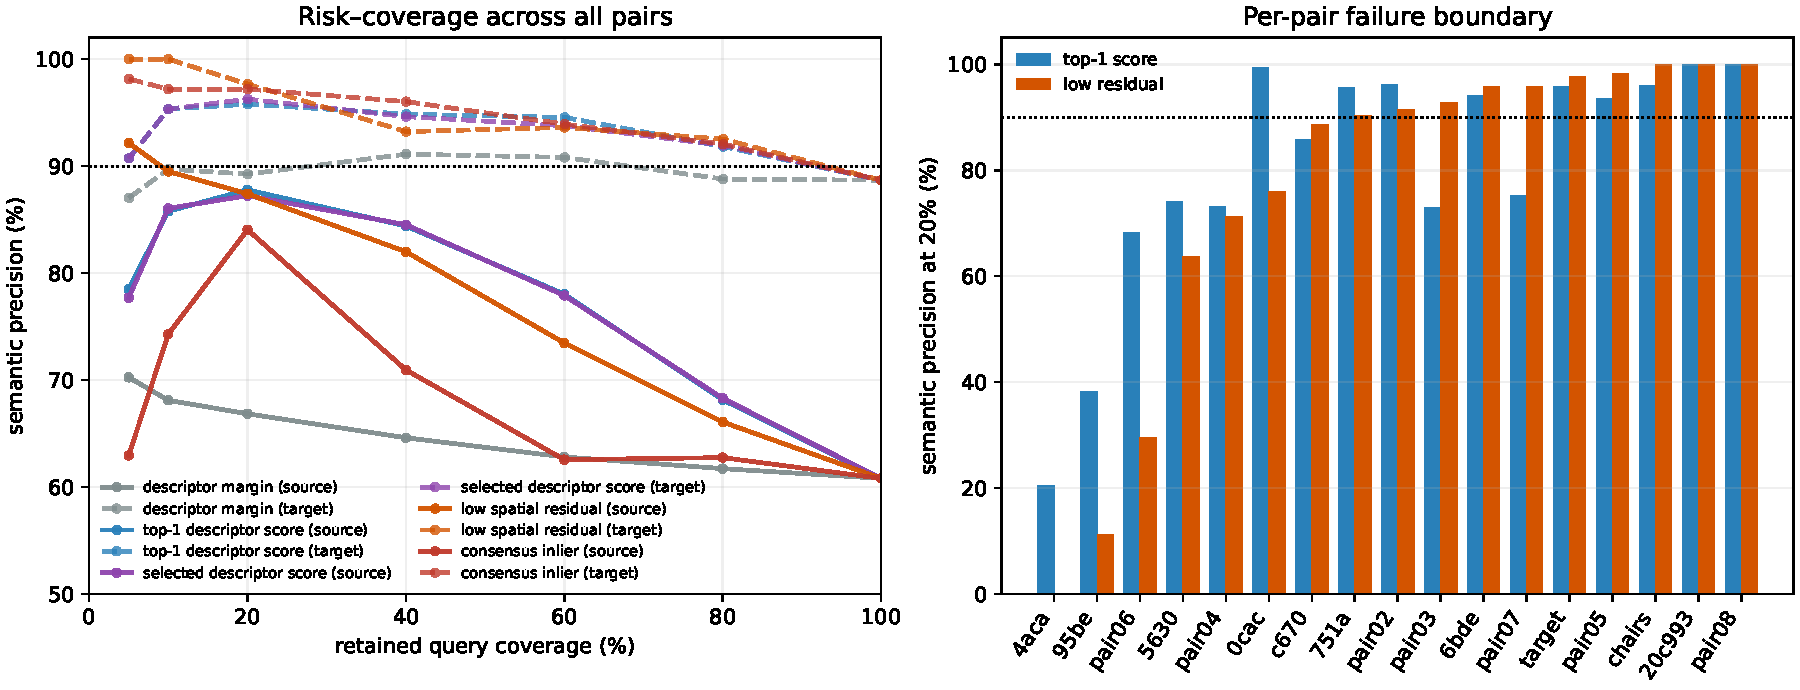
\includegraphics[width=0.98\textwidth]{selective_correspondence_overview.pdf}
\caption{Full selective audit. Left: source (solid) and target (dashed)
risk--coverage curves. Right: per-pair retained semantic accuracy at 20\% coverage;
the low bars for 4aca and 95be are candidate-availability/consensus failures,
not merely aggregate pose failures.}
\label{fig:risk}
\end{figure*}

\begin{figure*}[t]
\centering
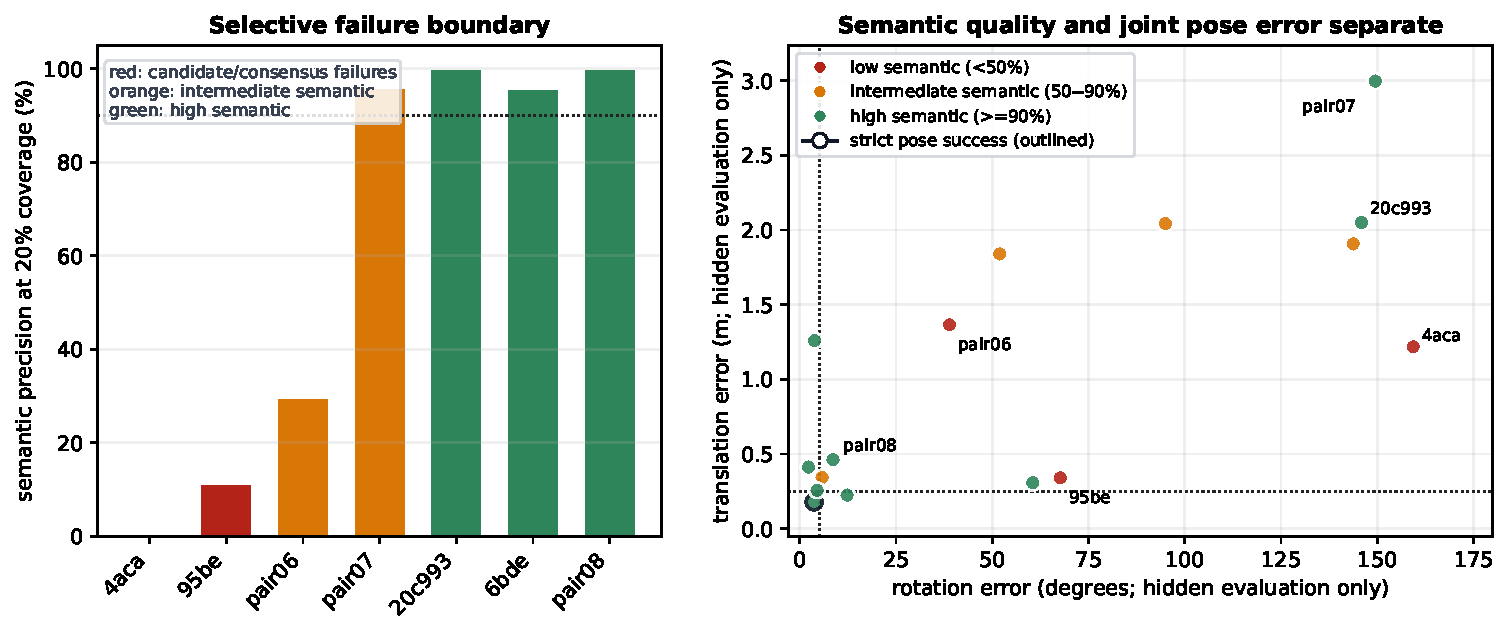
\includegraphics[width=0.98\textwidth]{failure_taxonomy.pdf}
\caption{Joint failure audit on source pairs. Left: at fixed 20\% coverage,
candidate-availability/consensus failures remain low even after residual
selection. Right: rotation and translation errors are shown jointly; dashed
lines mark the strict $5^\circ/0.25$~m pose gate. Colors are mutually
exclusive retained-semantic-accuracy bands, and marker outlines identify strict
pose successes, so a high-semantic but wrong-pose pair such as 6bde is visible.}
\label{fig:failure}
\end{figure*}

The failure taxonomy is important. In 4aca, only 19.5\% of evaluated queries
have any semantically correct top-20 candidate, and no correct semantic inlier
survives; it is a direct candidate-set failure. In 95be, 69.2\% have a
semantically correct candidate, but only 1.0\% of those candidate-hit queries
become correct inliers, exposing a wrong-consensus/pose failure. Other pairs,
including 20c993 and 6bde, can have high-semantic inliers while selecting an
incorrect global pose. These cases motivate reporting candidate availability,
semantic correctness, pose error, and abstention coverage as separate axes.
Figure~\ref{fig:failure} visualizes these failure families over the expanded
source audit.

\subsection{Cross-scan label transfer}
Table~\ref{tab:transfer} treats each selected match as a semantic and instance
label-transfer prediction. On the target, consensus inliers provide 85.5\%
semantic mIoU at 68.0\% coverage. The source-fit residual selector
raises conditional semantic mIoU to 89.5\% and conditional instance mIoU to
90.7\% at 22.1\% coverage. Over the fixed target query population, with
abstentions counted as false negatives, its semantic mIoU is 19.7\%.
The corresponding pooled conditional semantic mIoU is 61.2\%, while the
pair-macro conditional semantic mIoU is 67.3\%; the two values differ because
the former pools retained queries before taking the class mean and the latter
first computes one mIoU per pair. Both are conditional on retention and are
reported to avoid conflating them.
The downstream geometry-control audit in the supplement gives FCGF 64.2\%
semantic mIoU at 17.5\% target coverage and FPFH 82.8\% at 13.2\%; FPFH
uses voxelized points, so this is a diagnostic comparison rather than an
equal-density claim.

\begin{table}[t]
\centering
\caption{Cross-scan label transfer. Conditional mIoU is class-balanced over
retained queries; the fixed-query abstention-aware version is in the supplement.}
\label{tab:transfer}
\small
\begin{tabular}{lccc}
\toprule
Dataset / selector & Cov. & Sem. mIoU & Inst. mIoU \\
\midrule
Source / all & 100.0\% & 19.4\% & 19.3\% \\
Source / consensus & 30.4\% & 41.5\% & 39.0\% \\
Source / source-fit & 8.9\% & 61.2\% & 51.5\% \\
Target / all & 100.0\% & 67.4\% & 55.5\% \\
Target / consensus & 68.0\% & 85.5\% & 72.3\% \\
Target / source-fit & 22.1\% & 89.5\% & 90.7\% \\
\bottomrule
\end{tabular}
\end{table}

\section{Limitations and conclusion}

This is a selective correspondence study, not a universal registration or
efficiency claim. The frozen headline snapshot contains 17 availability-selected
reference/rescan relations (16 sources and one target), out of 1,004 relations
listed in the metadata. The exact IDs and inclusion scope are reported in the
supplement. Although scan UUIDs are distinct, physical-site overlap across
relations was not verified; pair-bootstrap intervals therefore describe
relation-level variation rather than confirmed independent-site uncertainty.
One held-out target cannot establish broad generalization. Applied without
refitting, the source-only residual gate
is not a guarantee outside this split; the present snapshot does not claim
external validation beyond the reported target.
FPFH and FCGF are geometry controls;
neither receives RGB evidence, and the FCGF result is reported as a control
rather than tuned for 3RScan. The current label-transfer task demonstrates
utility; downstream VLM task success and sparse-execution speedups remain
future work.

The evidence supports a narrower conclusion: the larger frozen transformer has
a higher final retained semantic-accuracy point estimate on the matched subset,
but the uncertainty interval includes zero and no pre-consensus candidate-layer
effect was isolated. Spatial consensus makes a useful high-accuracy retained
subset explicit, but neither component eliminates candidate-availability,
wrong-consensus, or wrong-pose hypotheses. Evaluating these axes separately yields a more reliable
and reproducible account of cross-scan correspondence under real RGB-D shift.

\begin{thebibliography}{14}
\bibitem{dinov2} M.-E. Oquab et al. DINOv2: Learning Robust Visual Features
without Supervision. \emph{TMLR}, 2024.
\bibitem{3rscan} K. Wald et al. 3RScan: The 3D Room Reconstruction Dataset.
\emph{ICCV}, 2019.
\bibitem{ransac} M. Fischler and R. Bolles. Random Sample Consensus.
\emph{CACM}, 1981.
\bibitem{fpfh} R. Rusu, N. Blodow, and M. Beetz. Fast Point Feature Histograms
(FPFH) for 3D Registration. \emph{ICRA}, 2009.
\bibitem{fcgf} C. Choy, J. Park, and V. Koltun. Fully Convolutional Geometric
Features. \emph{ICCV}, 2019.
\bibitem{3dmatch} A. Zeng et al. 3DMatch: Learning Local Geometric Descriptors
from RGB-D Reconstructions. \emph{CVPR}, 2017.
\bibitem{pointdsc} X. Bai et al. PointDSC: Robust Point Cloud Registration
Using Deep Spatial Consistency. \emph{CVPR}, 2021.
\bibitem{geotransformer} Z. Qin et al. Geometric Transformer for Fast and Robust
Point Cloud Registration. \emph{CVPR}, 2022.
\bibitem{regtr} Z. J. Yew and G. H. Lee. REGTR: End-to-End Point Cloud
Correspondences With Transformers. \emph{CVPR}, 2022.
\bibitem{dust3r} S. Wang, V. Leroy, Y. Cabon, B. Chidlovskii, and J. Revaud.
DUSt3R: Geometric 3D Vision Made Easy. \emph{CVPR}, 2024.
\bibitem{mast3r} V. Leroy, Y. Cabon, and J. Revaud. Grounding Image Matching
in 3D with MASt3R. \emph{ECCV}, 2024.
\bibitem{vggt} J. Wang, M. Chen, N. Karaev, A. Vedaldi, C. Rupprecht, and
D. Novotny. VGGT: Visual Geometry Grounded Transformer. \emph{CVPR}, 2025.
\bibitem{semreg} S. Fung, X. Lu, D. de Silva Edirimuni, W. Pan, X. Liu, and
H. Li. SemReg: Semantics Constrained Point Cloud Registration. \emph{ECCV}, 2024.
\bibitem{mlsemreg} S. Yan, P. Shi, and J. Li. ML-SemReg: Boosting Point Cloud
Registration with Multi-level Semantic Consistency. \emph{ECCV}, 2024.
\end{thebibliography}

\end{document}
